\documentclass[t,aspectratio=169]{beamer} % 使用16:9宽高比
\usetheme{Madrid} % 选择Madrid主题
\usecolortheme{default} % 使用默认颜色主题

% 设置字体
\usepackage[UTF8]{ctex}
\usefonttheme{structurebold} % 加粗结构字体

% 数学包
\usepackage{amsmath, amssymb, bm}
\usepackage{url}

% 图形包 (如果需要插入图片)
\usepackage{graphicx}
% \graphicspath{{./images/}} % 假设图片放在images文件夹

% 标题页信息
\title[7.1.误差曲面]{第7章：梯度下降}
\subtitle{第1节：误差曲面 (Error Surfaces)}
\author{《深度学习基础》课程小组}
% \institute{上海立信会计金融学院}
\date{\today}

\begin{document}

% 标题页
\frame{\titlepage}

% 目录页
\begin{frame}
    \frametitle{目录}
    \tableofcontents
\end{frame}

% ============================================================
% 第一部分：神经网络的参数设定
% ============================================================
\section{神经网络的参数设定}

\begin{frame}
    \frametitle{1. 从函数逼近到参数设定}
    \begin{itemize}
        \item 神经网络是一类\alert{非常广泛且灵活}的函数。
        \item 原则上，只要隐藏单元足够多，就能以任意精度逼近任何函数。
        \item 深度神经网络还能编码与\alert{层级化表示}对应的归纳偏置。
        \item 现在的问题：\alert{如何根据训练数据，找到合适的网络参数（权重和偏置）？}
    \end{itemize}
\end{frame}

\begin{frame}
    \frametitle{1.1 关键概念：归纳偏置与层级化表示}
    \begin{block}{归纳偏置 (Inductive Bias)}
        模型为了从有限数据中泛化而做出的一系列假设或偏好。\\
        例如：CNN 的归纳偏置是“平移不变性”——猫在图像左上角还是右下角，都是猫。
    \end{block}
    \begin{block}{层级化表示 (Hierarchical Representations)}
        数据特征被组织成从低级到高级、从简单到复杂的层次结构。\\
        例如：人脸识别中，底层提取边缘线条 $\rightarrow$ 中层组合成眼睛、鼻子 $\rightarrow$ 高层组合成完整人脸。
    \end{block}
    \begin{itemize}
        \item \alert{实验建议}：结合 MNIST 手写数字识别，把这两个概念串起来。
    \end{itemize}
\end{frame}

% ============================================================
% 第二部分：基于梯度的误差函数优化
% ============================================================
\section{基于梯度的误差函数优化}

\begin{frame}
    \frametitle{2. 为什么要用梯度？}
    \begin{itemize}
        \item 与回归和分类模型一样，我们通过\alert{优化误差函数}来选择模型参数。
        \item 误差函数可以用\alert{最大似然法}来定义。
        \item 直接评估误差函数值来最小化（如网格搜索）——\alert{效率非常低}。
        \item 更高效的方法：\alert{利用梯度信息}，即计算误差函数对网络参数的导数。
        \item 这就是为什么我们要求神经网络和误差函数都\alert{可微}。
    \end{itemize}
\end{frame}

\begin{frame}
    \frametitle{2.1 如何用最大似然构造误差函数？}
    \begin{enumerate}
        \item \textbf{写出似然函数}：假设样本独立同分布，
        \[
        L(\mathbf{w}) = \prod_{n=1}^{N} p(t_n | x_n, \mathbf{w})
        \]
        \item \textbf{取对数}：将乘积转化为求和，
        \[
        \ln L(\mathbf{w}) = \sum_{n=1}^{N} \ln p(t_n | x_n, \mathbf{w})
        \]
        \item \textbf{转化为误差函数}：最大化对数似然等价于最小化负对数似然，
        \[
        E(\mathbf{w}) = -\ln L(\mathbf{w}) = -\sum_{n=1}^{N} \ln p(t_n | x_n, \mathbf{w})
        \]
    \end{enumerate}
    \begin{itemize}
        \item 回归（高斯噪声）$\rightarrow$ 均方误差 (MSE)
        \item 二分类（伯努利分布）$\rightarrow$ 交叉熵损失 (Cross-Entropy)
    \end{itemize}
\end{frame}

\begin{frame}
    \frametitle{2.2 什么是直接误差函数评估？}
    \begin{itemize}
        \item \textbf{定义}：不使用梯度信息，仅通过反复“代入参数值 $\rightarrow$ 计算误差”来寻找最小值。
        \item \textbf{典型方法}：网格搜索 (Grid Search)、随机搜索 (Random Search)、Nelder-Mead 单纯形法。
        \item \textbf{为什么效率低？}
        \begin{itemize}
            \item 神经网络参数量巨大（数万到数百万）。
            \item 在高维空间中逐点评估，就像\alert{蒙着眼睛在山谷里找最低点}。
            \item 利用梯度，就像\alert{知道了脚下山坡的倾斜方向}，可以直接朝下坡方向大步前进。
        \end{itemize}
    \end{itemize}
\end{frame}

% ============================================================
% 第三部分：反向传播
% ============================================================
\section{反向传播}

\begin{frame}
    \frametitle{3. 反向传播：高效计算导数}
    \begin{itemize}
        \item 误差函数对网络中各参数的导数，可以用\alert{反向传播 (Backpropagation)} 高效计算。
        \item 核心思想：计算过程从后向前传递，类似于前向传播的“镜像”。
        \item \textbf{前向传播}：输入 $\rightarrow$ 逐层计算 $\rightarrow$ 得到预测 $\rightarrow$ 计算误差（保存中间变量）。
        \item \textbf{反向传播}：从误差开始 $\rightarrow$ 利用保存的中间变量 $\rightarrow$ 逐层回传局部梯度 $\rightarrow$ 得到所有参数的梯度。
    \end{itemize}
\end{frame}

\begin{frame}
    \frametitle{3.1 反向传播为什么高效？}
    \begin{itemize}
        \item \textbf{链式法则逐层分解}：
        \[
        \frac{\partial E}{\partial \text{某层参数}} = \frac{\partial E}{\partial \text{该层输出}} \times \frac{\partial \text{该层输出}}{\partial \text{该层输入}} \times \frac{\partial \text{该层输入}}{\partial \text{该层参数}}
        \]
        \item \textbf{避免重复计算}：从输出层向输入层逐层回传“误差信号”，每层只需与自己的局部导数相乘。
        \item \textbf{计算复杂度}：约等于一次前向传播的两倍，将指数级计算量降为线性级别。
    \end{itemize}
    \begin{block}{实验建议}
        用一个简单的两神经元网络，手动走一遍前向传播和反向传播的具体计算过程。
    \end{block}
\end{frame}

% ============================================================
% 第四部分：泛化与正则化
% ============================================================
\section{泛化与正则化}

\begin{frame}
    \frametitle{4. 泛化能力与正则化的重要性}
    \begin{itemize}
        \item 虽然似然用于定义误差函数，但神经网络优化的目标是\alert{在测试数据上取得良好泛化}。
        \item \textbf{经典统计学}：数据多、参数少，目标是\alert{精确拟合}，找到似然最大化的唯一最优解。
        \item \textbf{现代深度学习}：参数极多（甚至多于数据量），目标\alert{不是精确优化}。
        \item 学习算法本身的特性（如 SGD 的隐式正则化）以及显式正则化方法（Dropout、权重衰减）对泛化至关重要。
    \end{itemize}
\end{frame}

% ============================================================
% 第五部分：误差曲面的几何直观
% ============================================================
\section{误差曲面的几何直观}

\begin{frame}
    \frametitle{5. 权重空间与误差曲面}
    \begin{itemize}
        \item 将所有权重和偏置整合为一个向量 $\mathbf{w}$，通过优化误差函数 $E(\mathbf{w})$ 来训练。
        \item \textbf{权重空间 (Weight Space)}：若网络有 $W$ 个参数，则权重空间是 $W$ 维空间，每个点代表一组参数。
        \item \textbf{误差曲面 (Error Surface)}：误差函数 $E(\mathbf{w})$ 像地形的高低起伏。
        \item \textbf{优化本质}：在这个高维地形中寻找海拔最低的山谷（全局极小值或较好的局部极小值）。
    \end{itemize}
    \begin{figure}
        \centering
        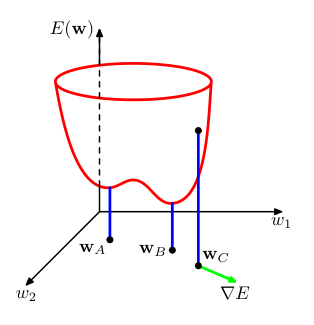
\includegraphics[width=0.2\textwidth]{figure7-1.png}
        \caption{误差函数 $E(w)$ 作为覆盖在权重空间之上的曲面。}
    \end{figure}
\end{frame}

% ============================================================
% 第六部分：驻点与梯度
% ============================================================
\section{驻点与梯度}

\begin{frame}
    \frametitle{6. 驻点与梯度的数学性质}
    \begin{itemize}
        \item 在权重空间中迈出一小步 $\delta\mathbf{w}$，误差变化为：
        \begin{equation}
        \delta E \simeq \delta\mathbf{w}^\mathrm{T} \nabla E(\mathbf{w})
        \tag{7.1}
        \end{equation}
        其中 $\nabla E(\mathbf{w})$ 指向误差增长最快的方向。
        \item 最小值出现在梯度为零的点：
        \begin{equation}
        \nabla E(\mathbf{w}) = \mathbf{0}
        \tag{7.2}
        \end{equation}
        \item 梯度为零的点称为\alert{驻点}，可分为极小值、极大值和鞍点。
    \end{itemize}
\end{frame}

\begin{frame}
    \frametitle{6.1 为什么要计算梯度？}
    \begin{itemize}
        \item \textbf{公式 (7.1)}：一阶泰勒近似。当 $\delta\mathbf{w}$ 与 $-\nabla E(\mathbf{w})$ 方向一致时，误差下降最快——这就是“梯度下降”名称的由来。
        \item \textbf{公式 (7.2)}：极值的一阶必要条件。找到“平地”（驻点），但可能是碗底、山顶或马鞍面。
        \item \textbf{深度学习中的挑战}：高维空间中鞍点远多于局部极小值。需要动量、Adam 等机制帮助跳出鞍点。
    \end{itemize}
\end{frame}

% ============================================================
% 第七部分：非线性与等效极小值
% ============================================================
\section{非线性与等效极小值}

\begin{frame}
    \frametitle{7. 误差曲面的非线性与等效极小值}
    \begin{itemize}
        \item 误差函数对权重和偏置具有\alert{高度非线性}依赖，存在许多梯度为零的点。
        \item 对于任何局部极小值 $\mathbf{w}$，通常还存在其他\alert{等效极小值}。
        \item 例如：具有 $M$ 个隐藏单元的两层网络，每个点属于一个包含 $M!\,2^M$ 个等效点的集合。
    \end{itemize}
    \begin{block}{为什么有这么多等效极小值？}
        \begin{itemize}
            \item \textbf{排列对称性 ($M!$)}：隐藏单元地位平等，交换任意两个单元的所有权重，网络输入输出关系不变。
            \item \textbf{符号对称性 ($2^M$)}：使用奇函数激活（如 tanh），将某单元所有输入输出权重同时取反，输出不变。
        \end{itemize}
    \end{block}
\end{frame}

% ============================================================
% 第八部分：全局与局部极小值
% ============================================================
\section{全局与局部极小值}

\begin{frame}
    \frametitle{8. 全局极小值与局部极小值}
    \begin{itemize}
        \item \textbf{全局极小值}：在整个 $\mathbf{w}$ 空间中误差函数最小的点。
        \item \textbf{局部极小值}：其他对应较高误差值的极小值点。
        \item 过去认为梯度法可能陷入较差的局部极小值。
        \item \alert{实践中并非如此}：大型网络在不同初始条件下都能达到性能相似的解。
    \end{itemize}
    \begin{block}{为什么深度学习不怕局部极小值？}
        \begin{itemize}
            \item 高维空间中\alert{鞍点远多于局部极小值}。
            \item 即使掉入局部极小值，其误差值往往接近，且处于\alert{平坦区域}，对应良好泛化能力。
        \end{itemize}
    \end{block}
\end{frame}

% ============================================================
% 第九部分：局部二次近似
% ============================================================
\section{局部二次近似}

\begin{frame}
    \frametitle{9. 局部二次近似与泰勒展开}
    \begin{itemize}
        \item 通过局部二次近似可以深入理解优化问题。
        \item $E(\mathbf{w})$ 在 $\tilde{\mathbf{w}}$ 附近的泰勒展开：
        \begin{equation}
        E(\mathbf{w}) \approx E(\tilde{\mathbf{w}}) + (\mathbf{w} - \tilde{\mathbf{w}})^\mathrm{T} \mathbf{b} + \frac{1}{2} (\mathbf{w} - \tilde{\mathbf{w}})^\mathrm{T} \mathbf{H} (\mathbf{w} - \tilde{\mathbf{w}})
        \tag{7.3}
        \end{equation}
        \item \textbf{梯度}：$\mathbf{b} \equiv \left.\nabla E\right|_{\mathbf{w} = \tilde{\mathbf{w}}}$
        \item \textbf{海森矩阵}：$\mathbf{H}(\tilde{\mathbf{w}}) \equiv \left.\nabla\nabla E(\mathbf{w})\right|_{\mathbf{w} = \tilde{\mathbf{w}}}$
        \item 梯度的局部近似：
        \begin{equation}
        \nabla E(\mathbf{w}) \approx \mathbf{b} + \mathbf{H}(\mathbf{w} - \tilde{\mathbf{w}})
        \tag{7.6}
        \end{equation}
    \end{itemize}
\end{frame}

\begin{frame}
    \frametitle{9.1 从 (7.3) 到 (7.6)：求梯度}
    对 (7.3) 式两边关于 $\mathbf{w}$ 求梯度：
    \begin{enumerate}
        \item 第一项 $E(\tilde{\mathbf{w}})$ 是常数，导数为 $\mathbf{0}$。
        \item 第二项 $(\mathbf{w} - \tilde{\mathbf{w}})^\mathrm{T} \mathbf{b}$ 是线性项，导数为 $\mathbf{b}$。
        \item 第三项 $\frac{1}{2} (\mathbf{w} - \tilde{\mathbf{w}})^\mathrm{T} \mathbf{H} (\mathbf{w} - \tilde{\mathbf{w}})$ 是二次型，导数为 $\mathbf{H}(\mathbf{w} - \tilde{\mathbf{w}})$。
    \end{enumerate}
    合并得：
    \[
    \nabla E(\mathbf{w}) \approx \mathbf{b} + \mathbf{H}(\mathbf{w} - \tilde{\mathbf{w}})
    \]
    \begin{block}{意义}
        \begin{itemize}
            \item (7.3) 用二次曲面近似原函数的“高度”。
            \item (7.6) 用切平面斜率近似原函数的梯度。
            \item 在牛顿法中，可通过求解 $\mathbf{H}\Delta\mathbf{w} = -\mathbf{b}$ 直接“跳跃”到近似极小值点。
        \end{itemize}
    \end{block}
\end{frame}

% ============================================================
% 第十部分：海森矩阵与二阶信息
% ============================================================
\section{海森矩阵与二阶信息}

\begin{frame}
    \frametitle{10. 海森矩阵与驻点分类}
    在极小值点 $\mathbf{w}^*$ 附近，$\nabla E = \mathbf{0}$，(7.3) 变为：
    \begin{equation}
    E(\mathbf{w}) = E(\mathbf{w}^*) + \frac{1}{2} (\mathbf{w} - \mathbf{w}^*)^\mathrm{T} \mathbf{H} (\mathbf{w} - \mathbf{w}^*)
    \tag{7.7}
    \end{equation}
    考虑海森矩阵的特征值方程：
    \begin{equation}
    \mathbf{H} \mathbf{u}_i = \lambda_i \mathbf{u}_i
    \tag{7.8}
    \end{equation}
    将 $(\mathbf{w} - \mathbf{w}^*)$ 展开为特征向量的线性组合：
    \begin{equation}
    \mathbf{w} - \mathbf{w}^* = \sum_i \alpha_i \mathbf{u}_i
    \tag{7.10}
    \end{equation}
    代入得：
    \begin{equation}
    E(\mathbf{w}) = E(\mathbf{w}^*) + \frac{1}{2} \sum_i \lambda_i \alpha_i^2
    \tag{7.11}
    \end{equation}
\end{frame}

\begin{frame}
    \frametitle{10.1 特征值与驻点类型}
    \begin{itemize}
        \item 若所有 $\lambda_i > 0$：$\mathbf{w}^*$ 是\alert{局部极小值}。
        \item 若所有 $\lambda_i < 0$：$\mathbf{w}^*$ 是\alert{局部极大值}。
        \item 若特征值有正有负：$\mathbf{w}^*$ 是\alert{鞍点}。
    \end{itemize}
    \begin{block}{直观理解}
        \begin{itemize}
            \item 特征向量 $\mathbf{u}_i$ 是误差曲面的“主轴”。
            \item 特征值 $\lambda_i$ 描述曲面在 $\mathbf{u}_i$ 方向上的弯曲程度。
            \item $\lambda_i > 0$：向上弯曲（碗底）；$\lambda_i < 0$：向下弯曲（山顶）。
        \end{itemize}
    \end{block}
\end{frame}

% ============================================================
% 第十一部分：正定矩阵与等高线
% ============================================================
\section{正定矩阵与等高线}

\begin{frame}
    \frametitle{11. 正定矩阵与局部极小值的充要条件}
    \begin{itemize}
        \item 矩阵 $\mathbf{H}$ 是\alert{正定}的，当且仅当：
        \begin{equation}
        \mathbf{v}^\mathrm{T} \mathbf{H} \mathbf{v} > 0, \qquad \text{对于所有 } \mathbf{v}
        \tag{7.12}
        \end{equation}
        \item 任意向量 $\mathbf{v} = \sum_i c_i \mathbf{u}_i$，则：
        \begin{equation}
        \mathbf{v}^\mathrm{T} \mathbf{H} \mathbf{v} = \sum_i c_i^2 \lambda_i
        \tag{7.14}
        \end{equation}
        \item $\mathbf{H}$ 正定 $\Leftrightarrow$ 所有特征值为正。
        \item \alert{局部极小值的充要条件}：梯度为零，且海森矩阵正定。
    \end{itemize}
\end{frame}

\begin{frame}
    \frametitle{11.1 等高线的几何直觉}
    \begin{itemize}
        \item 在以特征向量为基的新坐标系中，$E(\mathbf{w})$ 的等高线是\alert{轴对齐的椭圆}。
        \item 椭圆的轴长与对应特征值的\alert{平方根成反比}。
    \end{itemize}
    \begin{figure}
        \centering
        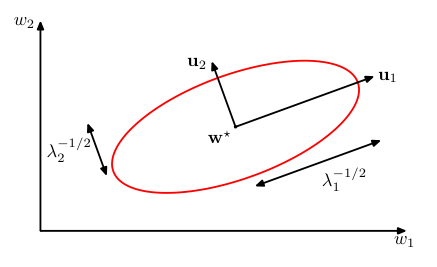
\includegraphics[width=0.3\textwidth]{figure7-2.png}
        \caption{在极小值 $w^*$ 附近，误差等高线为椭圆，其轴与海森矩阵的特征向量对齐。}
    \end{figure}
    \begin{itemize}
        \item $\lambda_i$ 越大，该方向上曲面越陡，等高线越扁。
        \item 若某些 $\lambda_i < 0$，等高线变为双曲线（鞍点特征）。
    \end{itemize}
\end{frame}

% ============================================================
% 第十二部分：总结
% ============================================================
\section{总结}

\begin{frame}
    \frametitle{12. 本节总结}
    \begin{itemize}
        \item 神经网络通过\alert{优化误差函数}来确定参数。
        \item \alert{梯度信息}使优化效率远高于直接评估。
        \item \alert{反向传播}高效计算所有参数的梯度，复杂度约等于两次前向传播。
        \item \alert{误差曲面}是覆盖在权重空间上的高维曲面，优化即寻找最低点。
        \item \alert{驻点}（梯度为零）分为极小值、极大值和鞍点。
        \item \alert{海森矩阵}的特征值决定驻点类型：全正为极小值，全负为极大值，有正有负为鞍点。
        \item 深度学习中，\alert{鞍点远多于局部极小值}，且局部极小值通常质量很高。
        \item \alert{局部二次近似}和\alert{正定矩阵}为理解优化提供了严格的数学工具。
    \end{itemize}
\end{frame}

% ============================================================
% 第十三部分：参考文献
% ============================================================
\section{参考文献}

\begin{frame}
    \frametitle{13. 参考文献}
    \begin{itemize}
        \item 教材：Bishop, C. M. \& Bishop, H. (2023). Deep Learning Foundations and Concepts. Springer Nature Switzerland AG.
        \item Bishop, C. M. (2006). Pattern Recognition and Machine Learning. Springer.
    \end{itemize}
\end{frame}

\end{document}